\chapter{Testing}
\label{chap:evaluation}

%%%%%%%%%%%%%%%%%%%%%%%%%%%%%%%%%%%%%%%%%%%%%%%%%%%%%%%%%%%%%%%%%%%%%%%%%%%%%%%%%%%%%%%%%%%%%%%%%%%%

A number of tests were ran to evaluate the correctness of the implemented robot control system. 

The robot control system was ran in its entirety on a high-end machine running Ubuntu Linux 12.04 LTS. Specifically, the machine has an \emph{Intel Core i7 3770K} clocked at \emph{4.5Ghz} paired with \emph{16GB} of memory. An attempt to run the control system on an \emph{Apple MacBook Pro} was made, which has an \emph{Intel Core i5 3239M} clocked at \emph{2.6Ghz} paired with \emph{8GB} of memory, but the machine could not achieve the performance necessary for good operation.

\begin{figure}[!h]
	\centering
	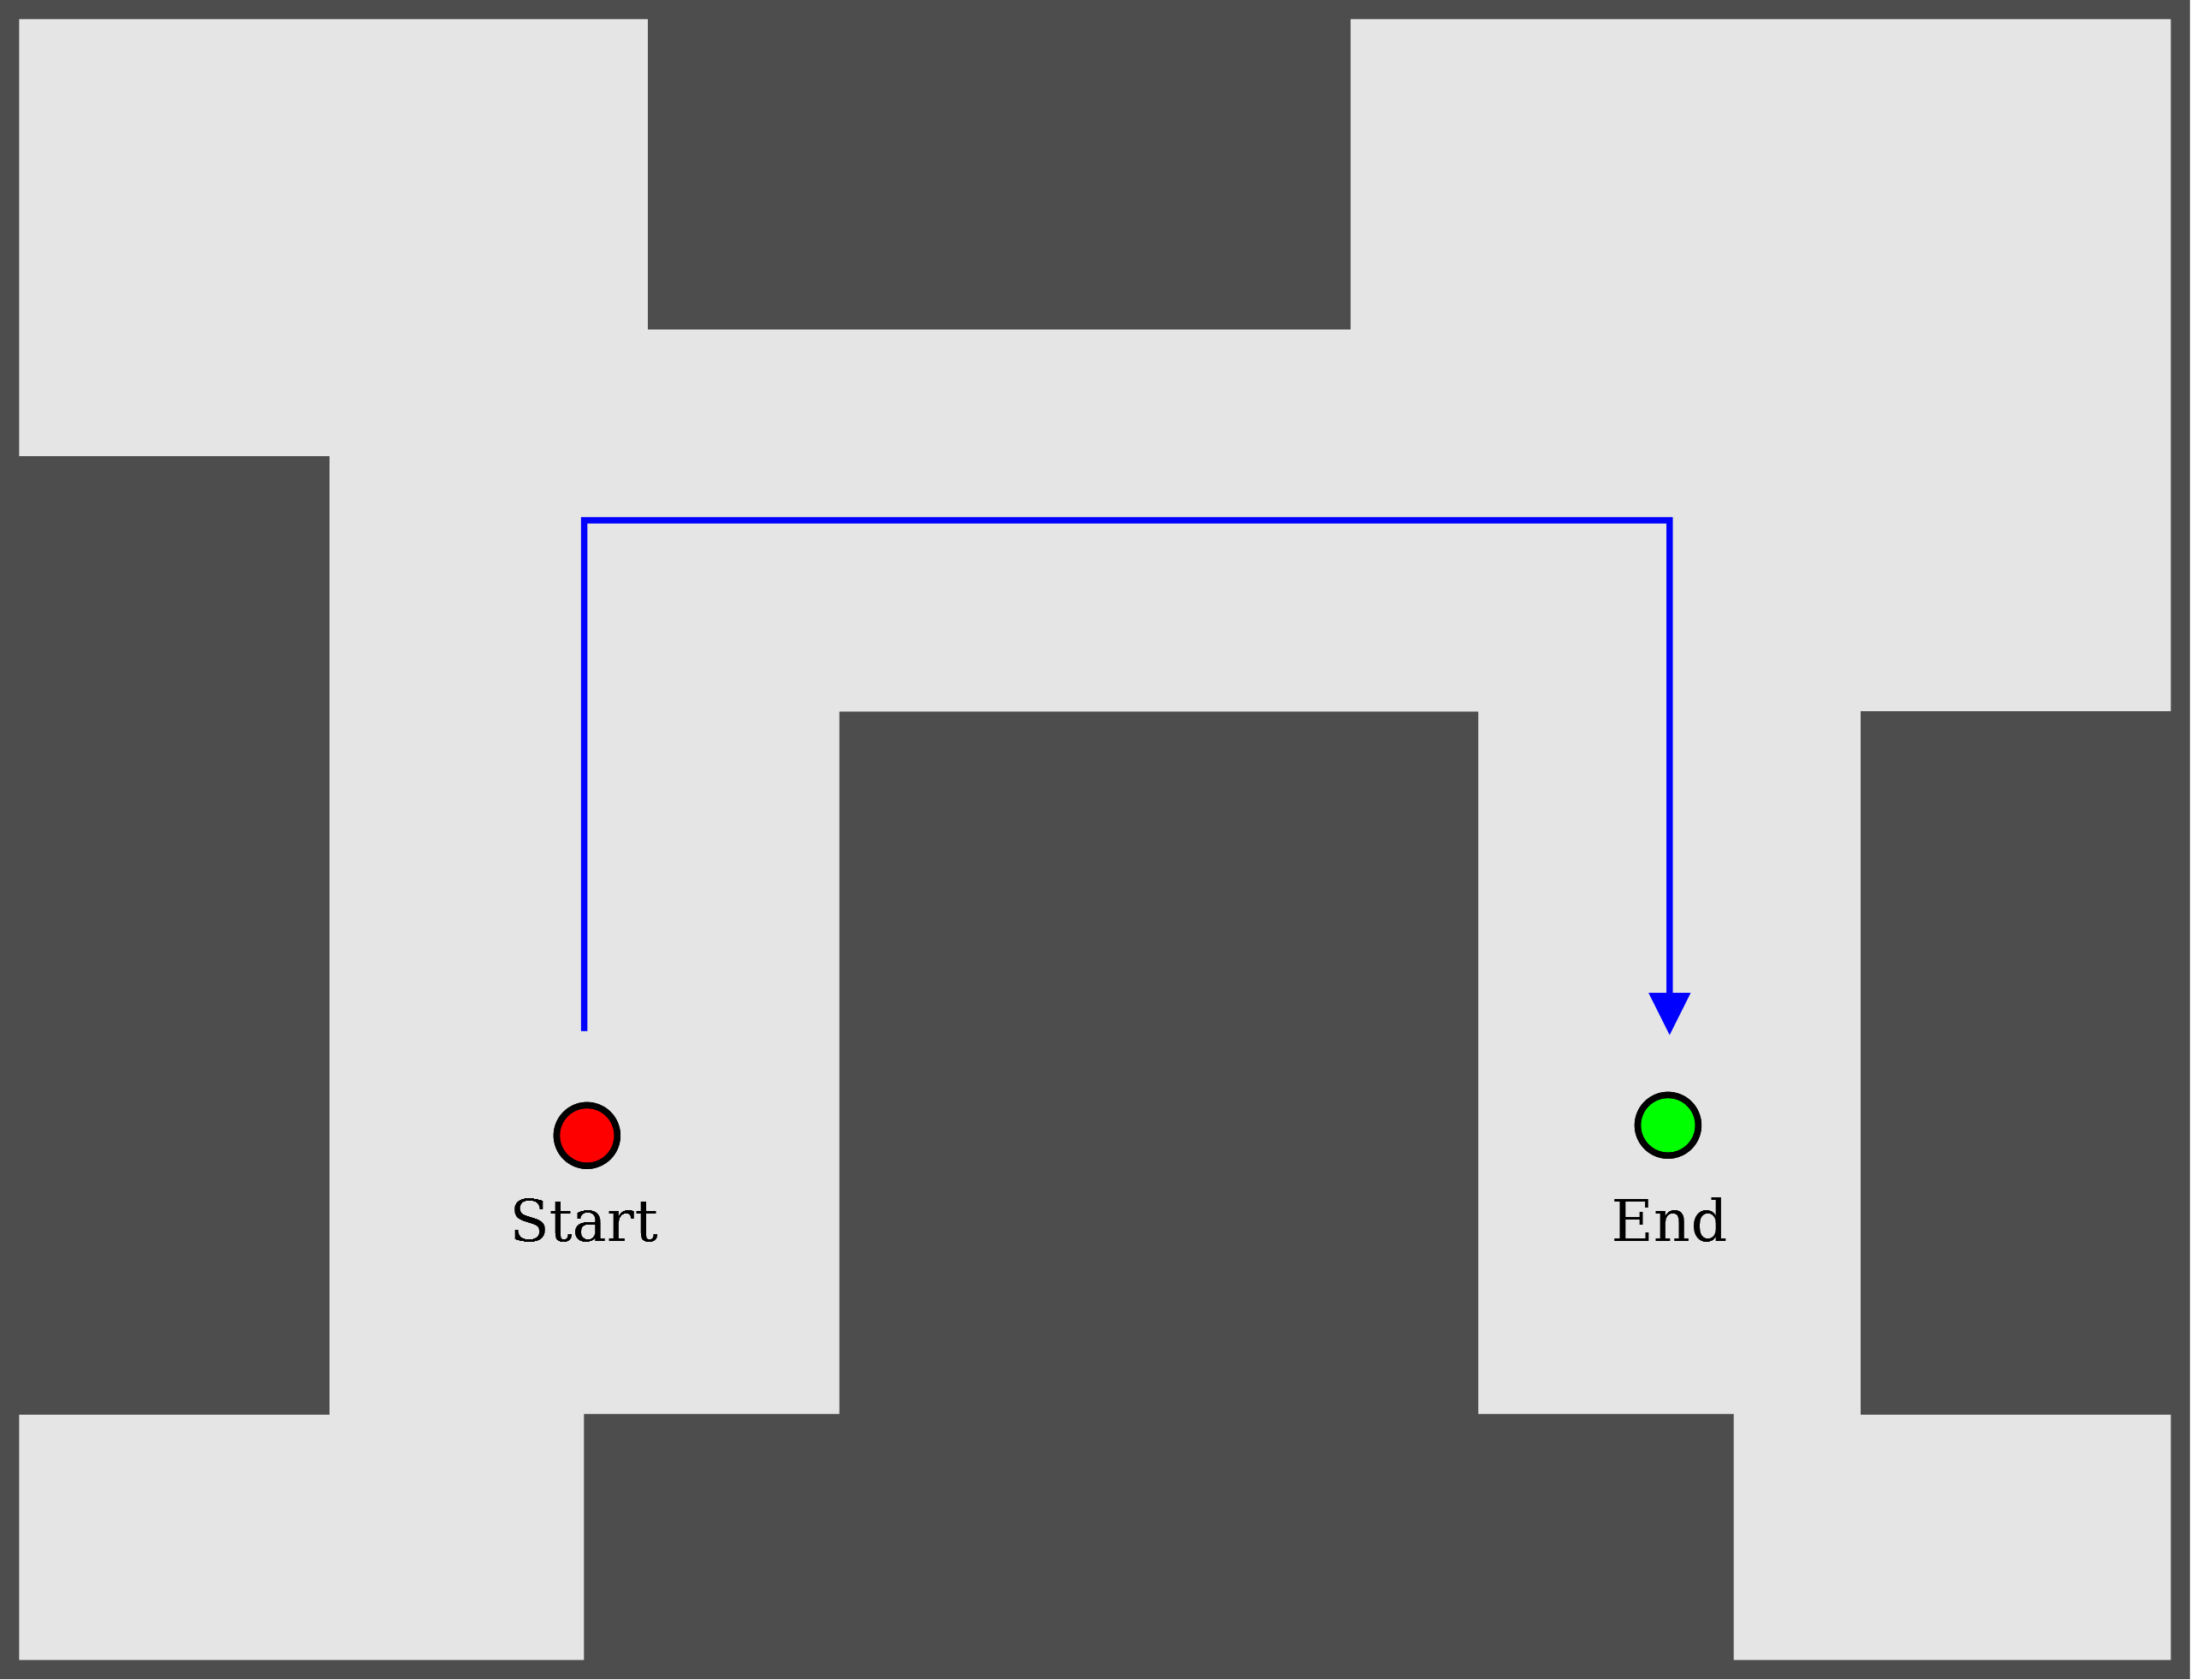
\includegraphics[width=12cm]{plan.png}
	\caption{A diagram of the general layout of the test environment (not to any particular scale). Darkened shapes indicate large obstacles that the robot must detect and avoid. The robot was placed at the starting point at the beginning of each test. The end point indicates the target goal for the navigational tests along with an ideal path.}
	\label{fig:eval_plan}
\end{figure}

Testing took place in a large bedroom environment as shown in \autoref{fig:eval_plan}. This environment contained a number of everyday obstacles with varying shapes, colours and textures. All tests were ran under ideal lighting conditions---i.e., full natural light---where possible. This ensured that the RGB-D sensor provided the highest quality images which would have a knock-on effect for the visual locomotory and mapping subsystems.

\section{Hardware Interaction}

\subsection{RGB-D Camera Driver}

The RGB-D camera driver, provided by the \texttt{openni2\_driver} and \texttt{openni2\_launch} packages

\subsection{Servo Driver}

To test the servo driver for the system, which is implemented as a custom \texttt{servo\_controller} node, we ran the following experiments. Each experiment was implemented as a custom node would would then be ran alongside the driver nodes to execute the test. Correctness of results were determined by visual observation---i.e., looking to see if joints moved as intended. 

\subsubsection{Rotation of a Single Servo}

This first test was designed to confirm correct behaviour when moving only one servo at a time. To elaborate further, this test aimed to check the following:

\begin{description}[labelindent=\parindent]
	\item[Hardware Communication] \hfill \\
	If the servo controller was receiving any of the serial output sent by the \texttt{servo\_controller} node whatsoever, the on-board indication LED would flash with each message. This would have shown that the servo controller is receiving serial output as intended. No flashing LED would have indicated some general issue with the serial communication systems.

	\item[Topic Reception] \hfill \\
	If the \texttt{servo\_controller} node was receiving \texttt{ServoCommand} messages sent on its \texttt{direct} topic, we expected some sort of change in system state in general---even if that involved the node crashing. No change would have indicated a problem with the topic subscriber within the node.

	\item[Index, Angle \& Duration Conversion] \hfill \\
	Should the formulae from converting from the units specified in the \texttt{ServoCommand} message to those specified by the servo controller's protocol be correct, we would have expected the specified servo to move the correct angle over the correct duration. Any deviation from this would have indicated some mathematical error in the formulae.
\end{description}

To implement this test, a \texttt{servo\_controller\_test\_single} node was created. This node requests four movements from each servo sequentially in a continuous loop at various angles and durations, pausing for one second between each. A listing of these movements is shown in \autoref{fig:servo_controller_eval}.

\begin{figure}[!h]
	\centering
	\begin{tabular}{ c c c }
		\toprule
		\textbf{Movement} & \textbf{Angle} & \textbf{Duration} \\
		\midrule

		$1$ &
		$90$\textdegree{} &
		$1.00$s \\

		$2$ &
		$180$\textdegree{} &
		$0.25$s \\

		$3$ &
		$0$\textdegree{} &
		$0.50$s \\

		$4$ &
		$90$\textdegree{} &
		$0.75$s \\
		\bottomrule
	\end{tabular}
	\caption{A listing of movements made for each servo in the single servo rotation test. These movements are applied to each servo in a continuous loop with a one second delay between each movement.}
	\label{fig:servo_controller_eval}
\end{figure}

The \texttt{servo\_controller} node and \texttt{servo\_controller\_test\_single} node were launched and the robot observed. Prior to this, the robot was placed upon a pedestal to ensure that the limbs could rotate freely without unintentionally moving the robot. As expected, each servo rotated as intended to the correct angles and durations, thus showing the implementation was functional as required.

\subsubsection{Simultaneous Rotation of Multiple Servos}

The second test was designed to confirm correct behaviour in the case of multiple servos being moved simultaneously---i.e., in the case where movement is requested for a number of servos such that the movement durations overlap. This was an essential requirement as no walk gaits would be possible without.

To implement this test, the \texttt{servo\_controller\_test\_single} node from the previous test was adapted to create a new \texttt{servo\_controller\_test\_multiple} node. This node performed the same set of movements but on all servos simultaneously rather than sequentially.

The \texttt{servo\_controller} node and \texttt{servo\_controller\_test\_double} node were launched and the robot observed, while the robot was placed on a pedestal as before. It was from this test that the necessity for a small delay between each serial communication was discovered. Without this delay, servos would either not rotate whatsoever or abort their requested rotation part-way through. During this, the indication LED on the servo controlled would also light up solidly, rather than flash as it does during normal operation. It was presumed that this meant there was some sort of communication error, perhaps as commands were being sent too quickly for the on-board microcontroller to process them. After adding an delay of $0.1$s, the problem immediately subsided. This was further reduced to a minimum delay of $0.003$s by trial-and-error, preventing any knock-on effects for commanding nodes. As mentioned in the implementation section for the \texttt{servo\_controller} node, no source code is available for the microcontroller software so no further diagnosis can be made. 

Following this modification, the test ran as intended, thus showing the implementation was functional as required.

\section{Locomotion}

These experiments were created to evaluate that the systems designed to handle locomotion operated correctly.

\subsection{Limb Controller}

\subsection{Limb Calibration Tool}

The implementation of the limb calibration tool is fairly trivial and was used throughout the evaluation of the control system and as such, no particularly rigorous testing was performed. Testing was performed throughout the implementation process and the node was found to work as intended. Generally, the joint servos had to be re-calibrated during each session of operation, as the particular servos used are rather inaccurate. A number of realisations came about during its use.

In particular, it was found that achieving an accurate calibration through manual manipulation was essentially impossible. There are no markings on the robot with which the current angles of joints can be compared, so calibration was usually done by eye alone. Using a measuring implement, such as a protractor, was also infeasible as the physical geometry of the robot prevents such devices from aligning correctly with the servo axles. This issue could be alleviated by adding additional sensors on the robot---e.g., gyroscopes and accelerometers---such that calibration could be performed automatically or to, at the very least, give some notion of the stability of the robot.

Additionally, it was found that the servos would not rotate by small increments but only when it had reached a certain threshold away from its current position---e.g., if a servo is currently at $90$\textdegree{} then it will not rotate immediately until a rotation of $\pm2$\textdegree{} is requested whereupon it will ``snap'' into position. The particular threshold seemed to vary wildly depending on the particular servo \emph{and} its position. This ramifications of this were such that while a limb may seem calibrated, it could in fact be out of alignment by this threshold. This would only become apparent when larger rotations were made.

In general, both of these issues could be solved be utilising more accurate (and accordingly more expensive) servos---software can only correct for hardware problems up to a point.

\subsection{Tripod Gait Walker}

Maximum speed constraints.

Walk cycle (linear).

Walk cycle (rotation).

Walk cycle (combination). 

\section{Sensing}

These experiments were created to evaluate that the systems could interpret the world around the robot via the supplied sensory input.

\subsection{Visual Odometry}

Visual odometry (manual movement of camera).

Visual odometry (walk cycle).

Mapping (while walking).

Visual odometry drift. Difficulty with stationary rotation. Interesting reaction to mirrors. No resync if location is lost.

\subsection{Mapping}

\begin{figure}[!h]
	\centering
	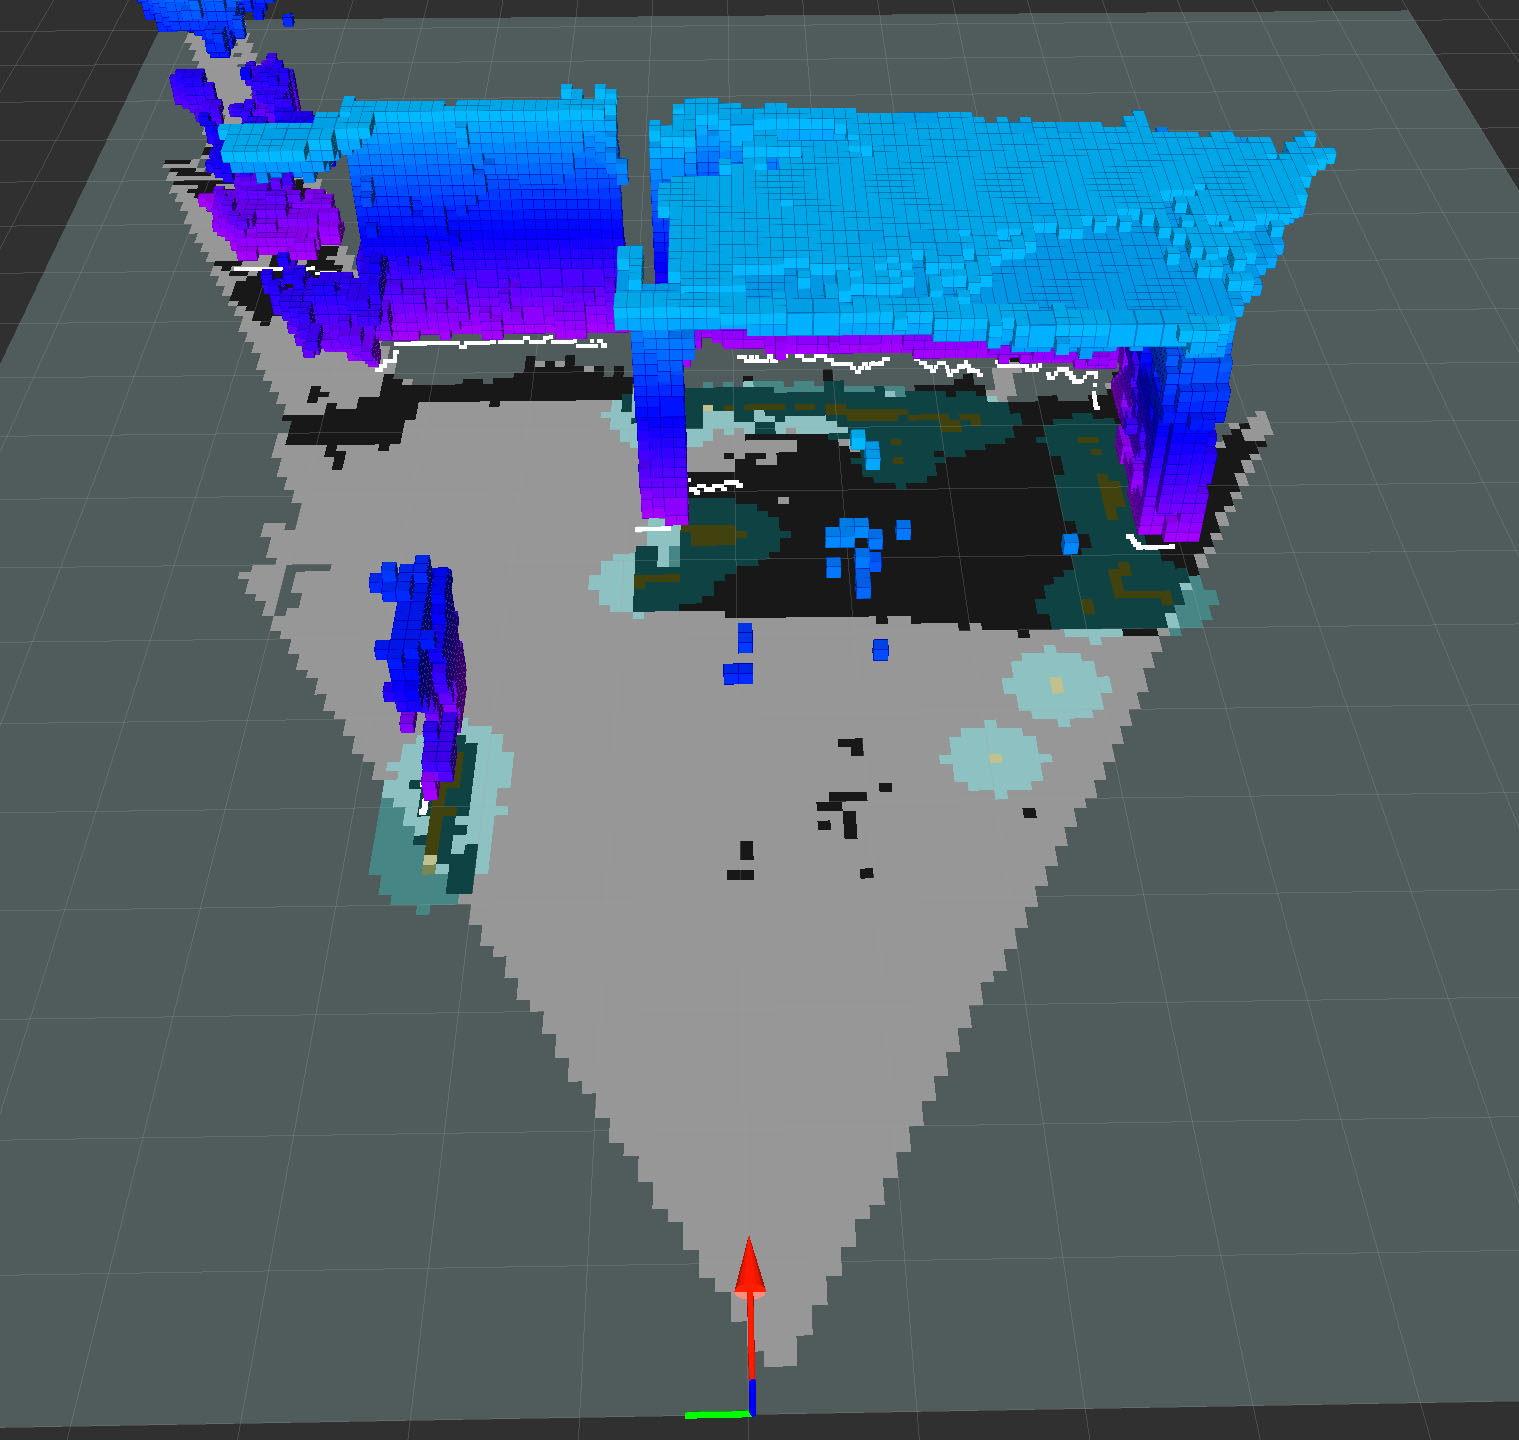
\includegraphics[width=12cm]{eval_map1.jpg} \\
	\vspace{2pt}
	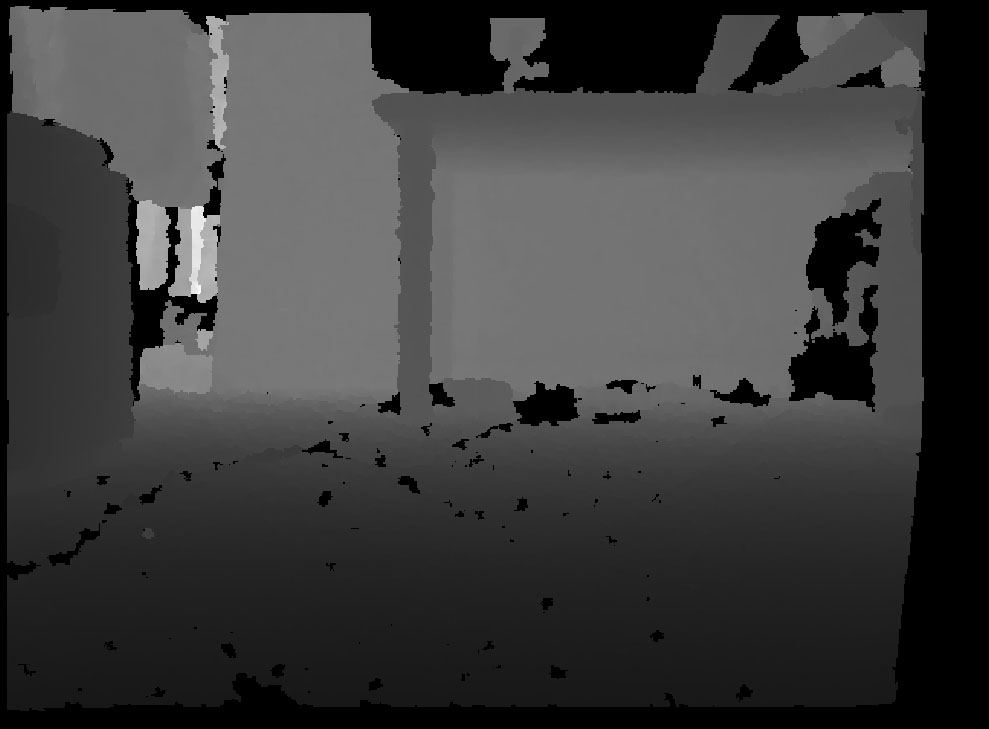
\includegraphics[width=8cm]{eval_rgbd3.jpg}
	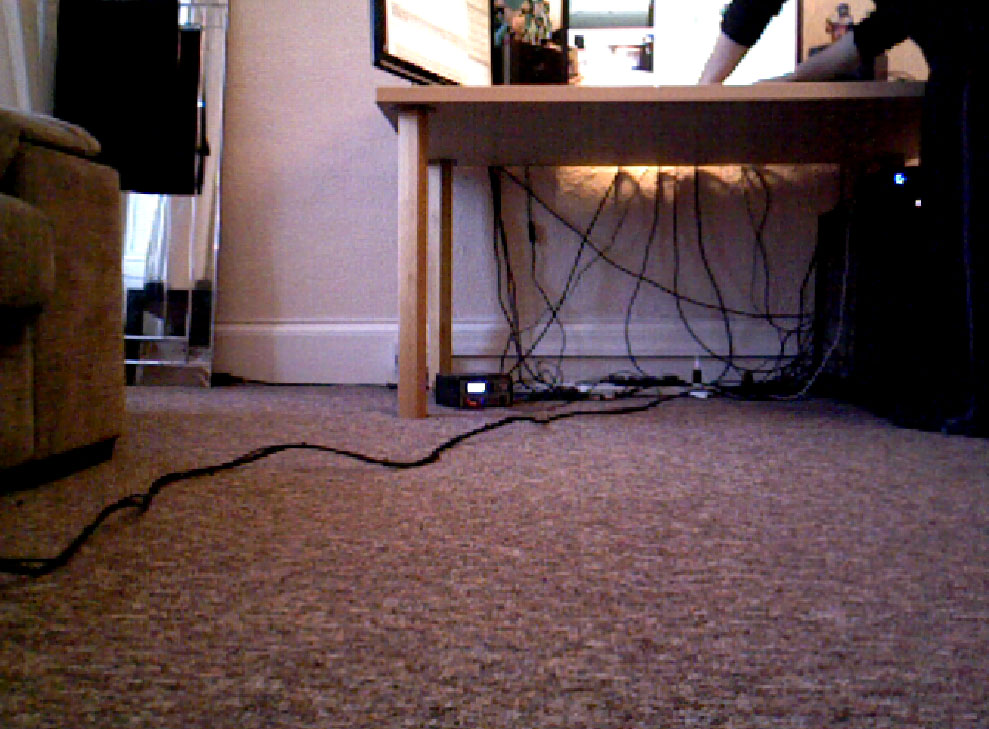
\includegraphics[width=8cm]{eval_rgbd4.jpg}
	\caption{A display of the generated map a few seconds after the robot control system has started along with the direct colour (bottom left) and depth (bottom right) outputs from the RGB-D camera. The shape of the desk and wall directly in front of the robot, as seen in the colour image, can clearly be seen in the resulting map.}
	\label{fig:eval_map_bag}
\end{figure}

\begin{figure}[!h]
	\centering
	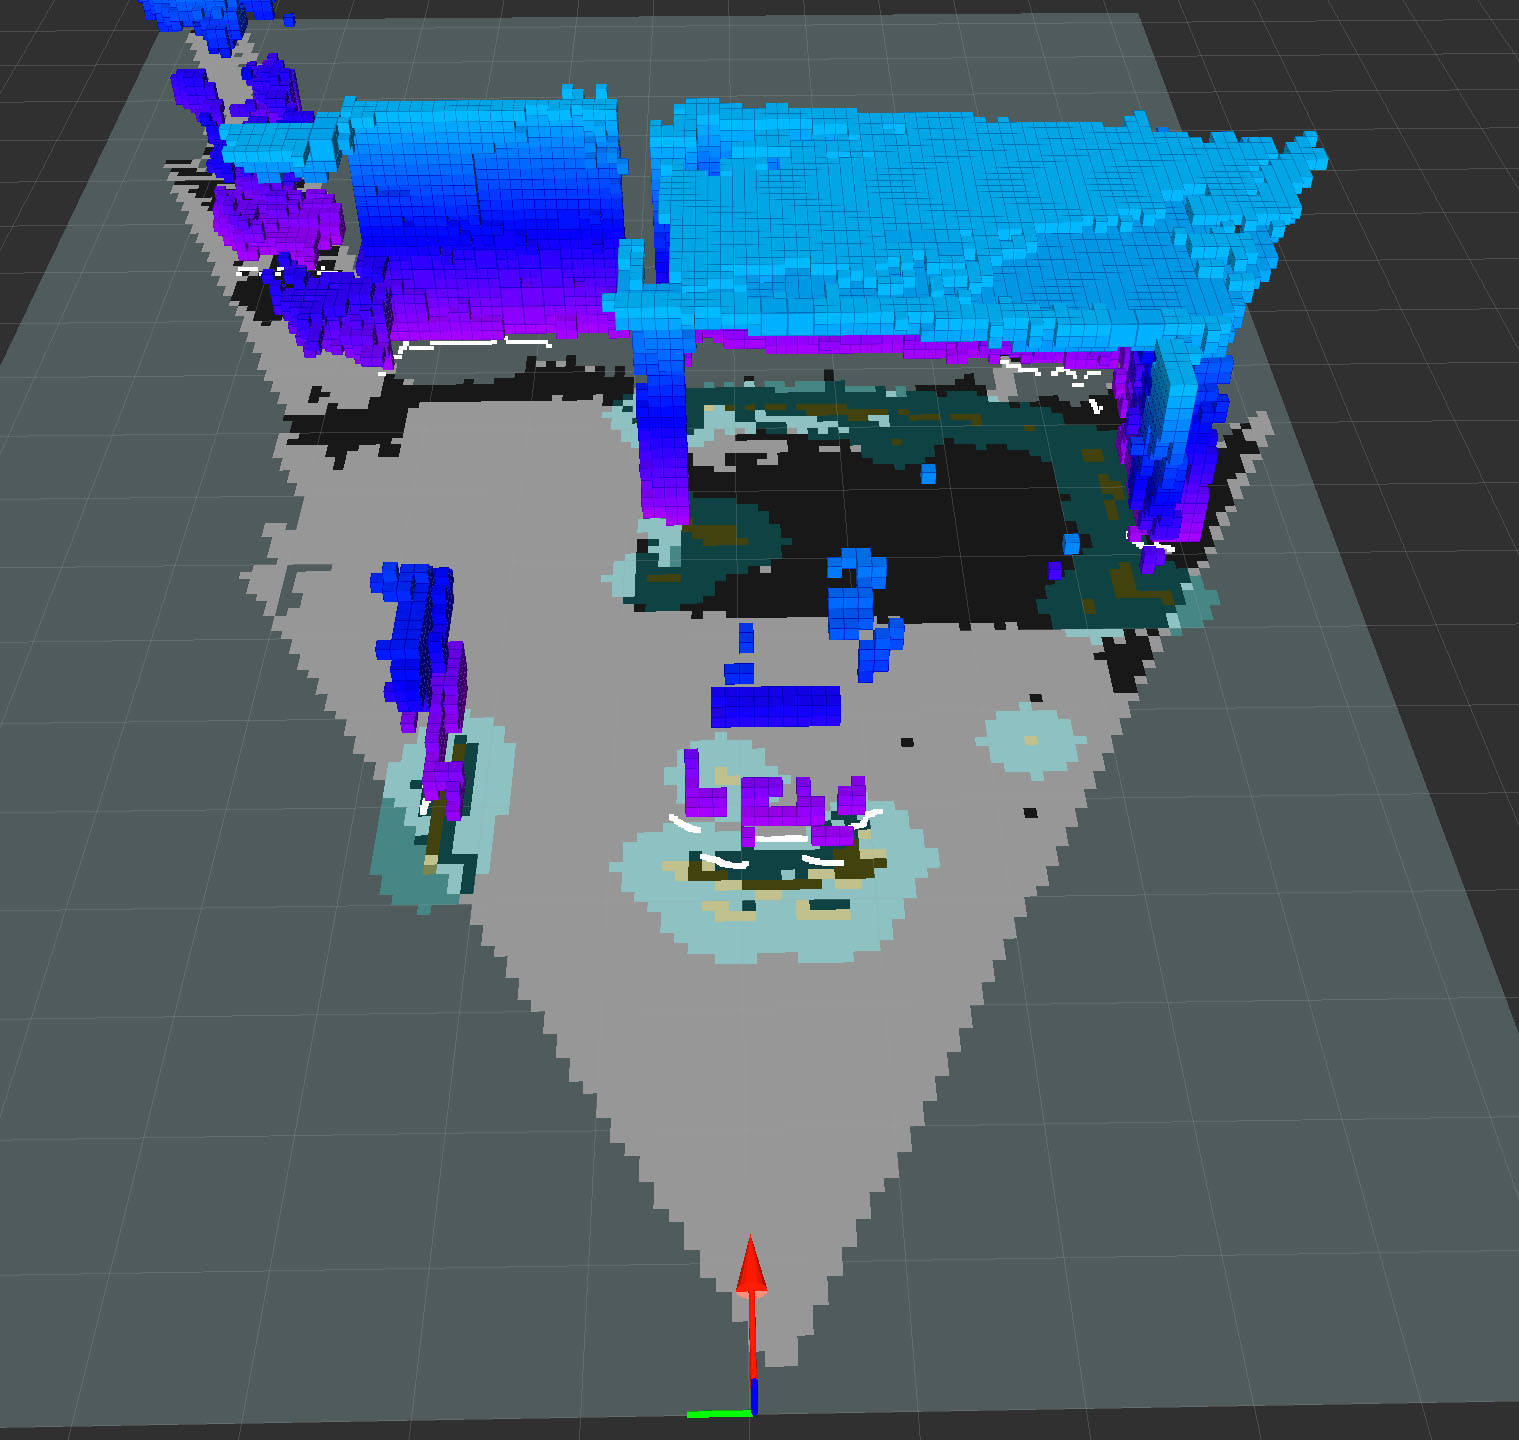
\includegraphics[width=12cm]{eval_map2.jpg} \\
	\vspace{2pt}
	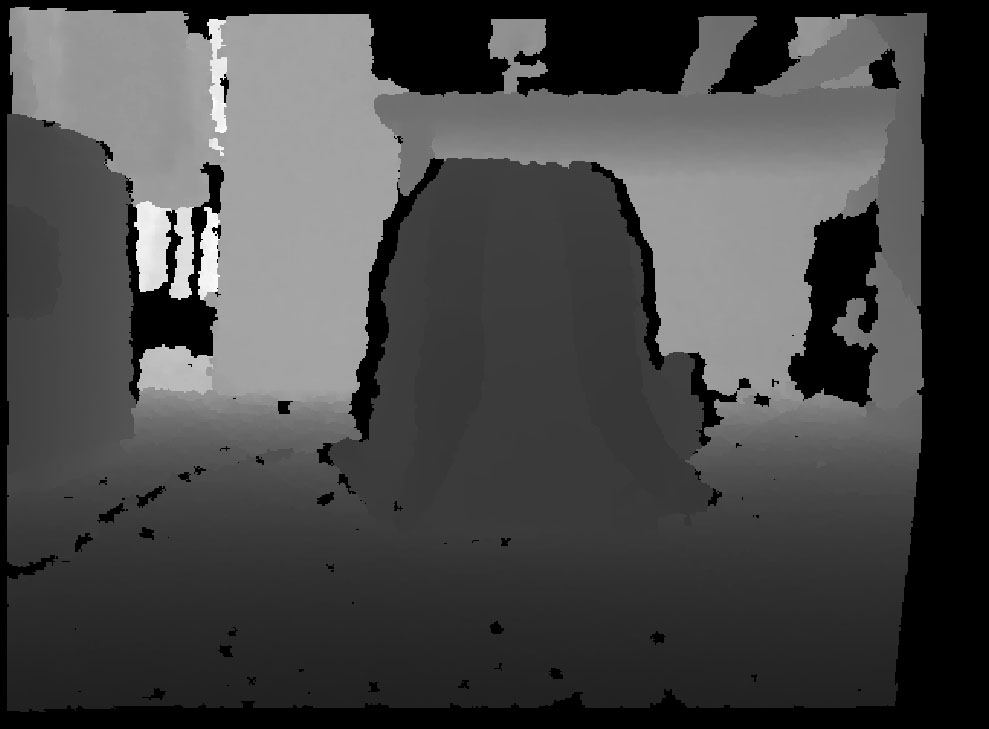
\includegraphics[width=8cm]{eval_rgbd1.jpg}
	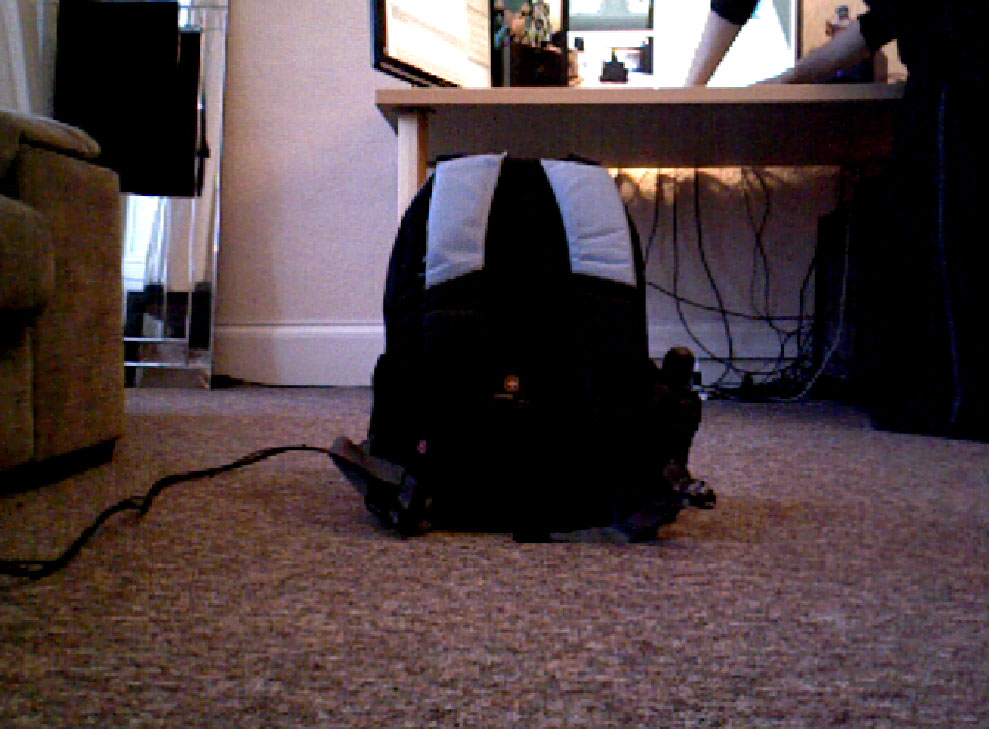
\includegraphics[width=8cm]{eval_rgbd2.jpg}
	\caption{A display of the generated map after an obstacle has been placed in front of the robot---a backpack in this case---along with the direct RGB (bottom left) and depth (bottom right) outputs from the RGB-D camera. The resulting blocks from the bag can be seen on the map. Notably, the bag appears as a rather patchy grouping of blocks but would still be enough to trigger any avoidance routines from the navigation system.}
	\label{fig:eval_map_nobag}
\end{figure}

\begin{figure}[!h]
	\centering
	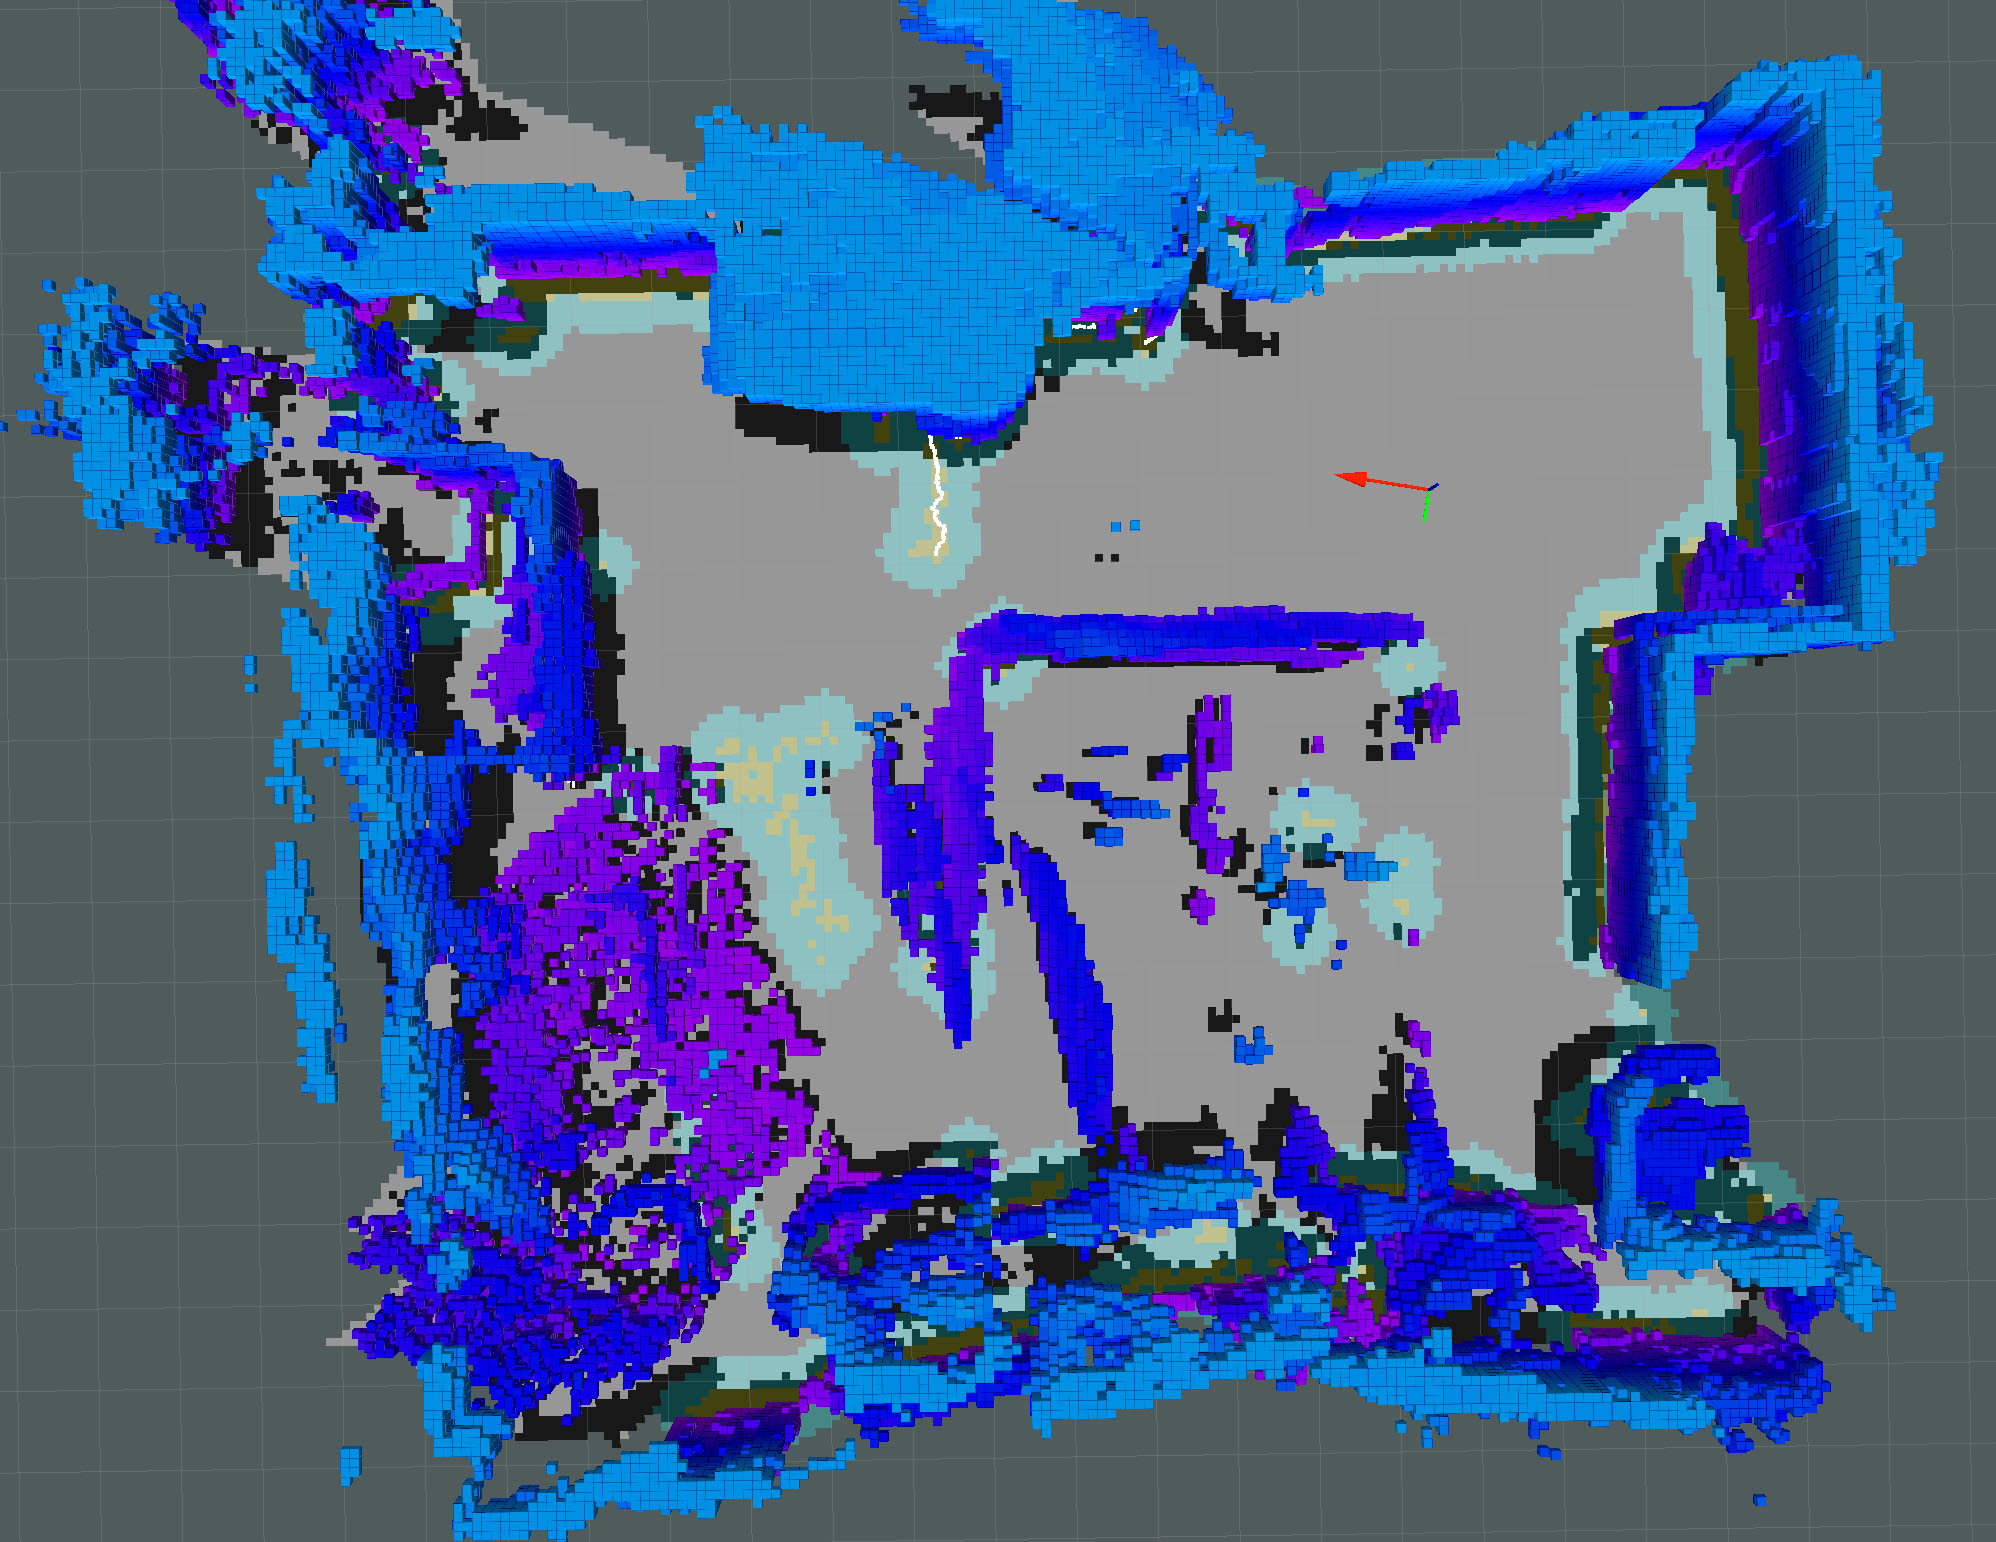
\includegraphics[width=16cm]{eval_map3.jpg}
	\caption{A display of the generated map after the robot has had a tour around the environment, as provided by RViz. It can be seen that the mapping system correctly generated a reasonable facsimile of the surrounding environment, however there is a large amount of distortion due to the drift from the visual locomotory system. Additionally, a rather large patch of the floor (bottom left, specifically) has been detected as an obstacle. As an aside, a strange effect results from the mirror that sits in the corner of the environment (top left, specifically).}
	\label{fig:eval_map_room}
\end{figure}

Mapping (stationary).

Mapping (object in front).

Mapping is awesome all of the time, ruined by visual odometry.

\section{Navigation}

These experiments were created to evaluate that the systems could navigate autonomously using the interpreted sensory information.

Navigation accuracy. (no obstacles, straight line)

Navigation accuracy. (obstacle in way, curved path)

Obstacles in way during navigation.

It works alright, I guess.